\section{CƠ SỞ LÝ THUYẾT}

Chương này trình bày toàn bộ nền tảng lý thuyết cốt lõi về Mô hình Mạng Zero Trust theo chuẩn NIST SP 800-207 và Khung trưởng thành 5 trụ cột CISA. Chương đi sâu phân tích sơ đồ kiến trúc tổng thể, mô tả chi tiết 5 luồng nghiệp vụ y tế cốt lõi (BF-01 đến BF-05) cùng ma trận phân quyền RBAC chi tiết. Đồng thời, chương giải thích cụ thể lý do tại sao lựa chọn và mục đích sử dụng của từng công nghệ trong hệ thống.

\subsection{Tổng quan về Mô hình Kiến trúc Zero Trust}

Kiến trúc Zero Trust dựa trên khung hướng dẫn NIST SP 800-207 thiết lập một nguyên tắc bảo mật căn bản là loại bỏ hoàn toàn niềm tin ngầm định theo vị trí kết nối vật lý. Dù người dùng truy cập từ mạng LAN nội bộ bệnh viện hay từ mạng Internet bên ngoài, mọi yêu cầu truy cập đều phải trải qua quá trình kiểm tra danh tính và cấp quyền liên tục.

Khung trưởng thành Zero Trust của Cơ quan An toàn An ninh mạng và Hạ tầng Mỹ (CISA) phân chia mô hình phòng thủ thành 5 trụ cột chính nhằm đảm bảo tính bao quát toàn diện bao gồm: Identity (Danh tính), Devices (Thiết bị), Networks (Mạng), Applications and Workloads (Ứng dụng) và Data (Dữ liệu), kết hợp với năng lực giám sát tập trung Visibility and Analytics.

\begin{figure}[H]
    \centering
    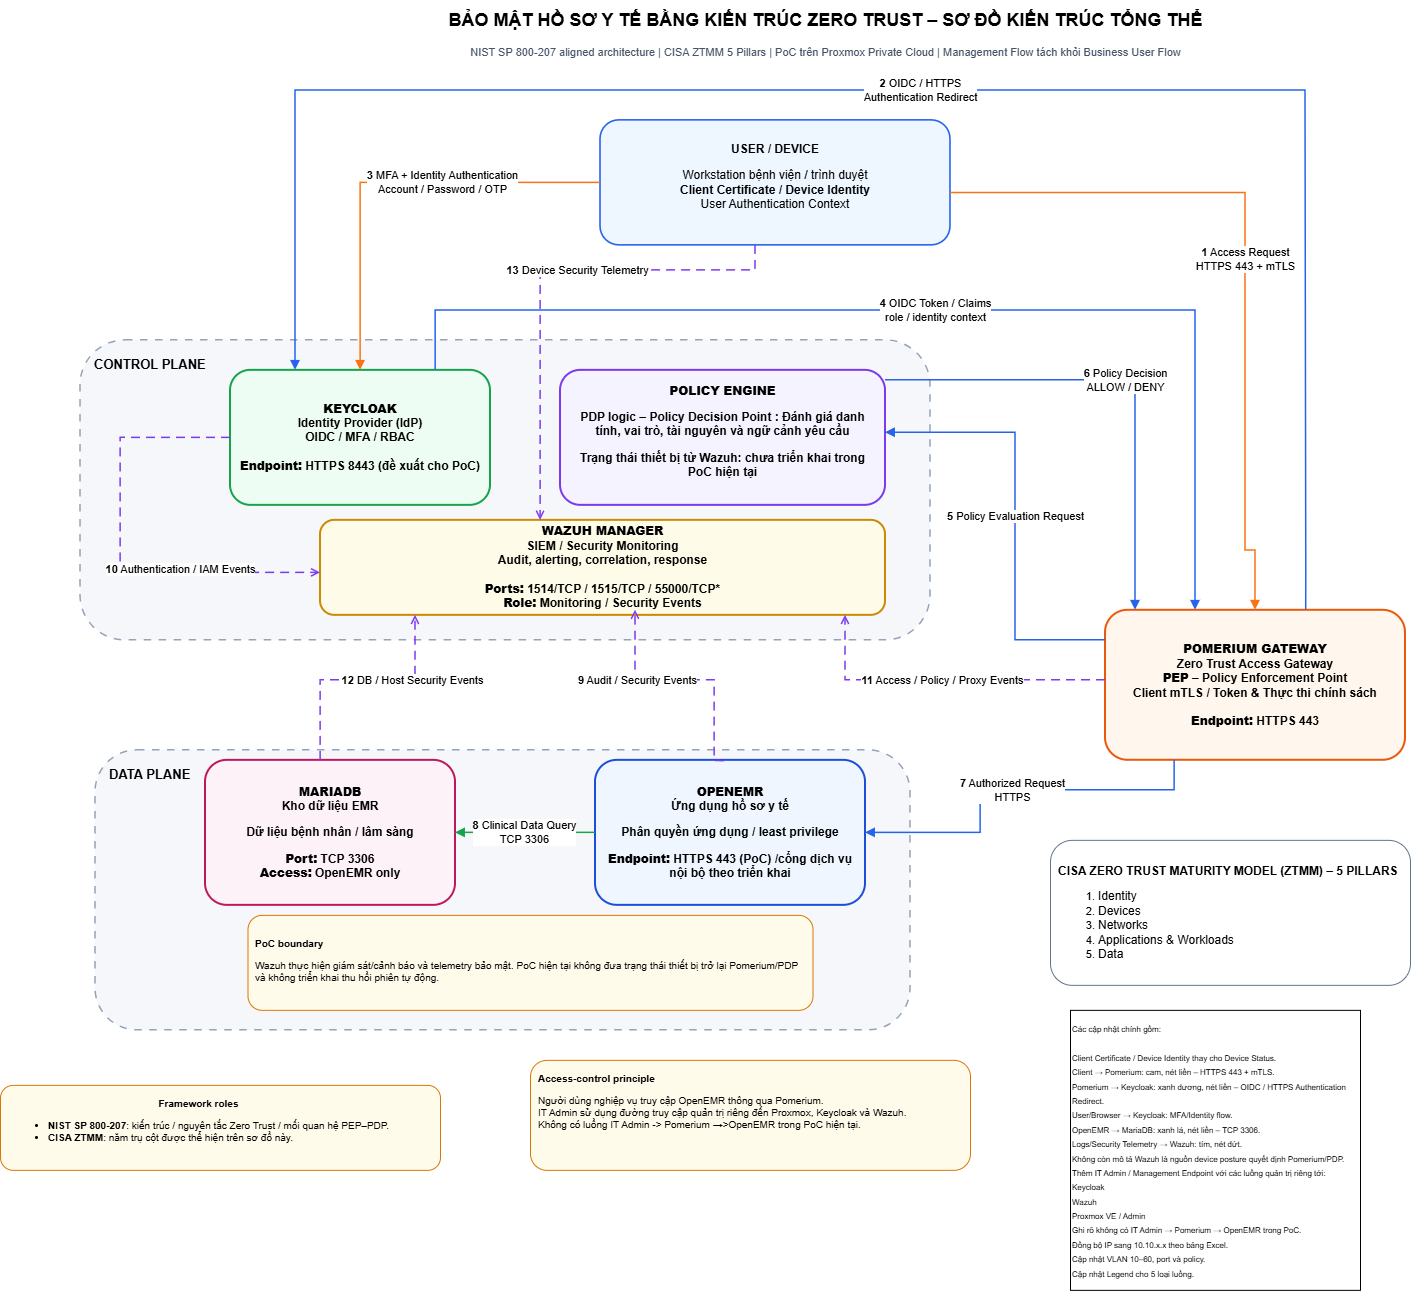
\includegraphics[width=0.95\textwidth]{image/zero_trust_overall_architecture_v2-Zero Trust Architecture.drawio.png}
    \caption{Sơ đồ kiến trúc tổng thể mô hình Zero Trust bảo mật Hồ sơ Y tế}
    \label{fig:overall_architecture}
\end{figure}

\subsubsection{Giải thích Chi tiết Sơ đồ Kiến trúc Tổng thể Mô hình Zero Trust (Hình 2.1)}

Sơ đồ kiến trúc tổng thể thể hiện mối quan hệ tương tác giữa 4 vùng thành phần chính: Vùng người dùng (Users/Devices), Vùng điều khiển truy cập (Access Control), Vùng ứng dụng \& dữ liệu (App \& Database), và Vùng giám sát an ninh (Security Monitoring).

Tạo tầng gác cổng uỷ quyền danh tính (Identity-Aware Proxy - Pomerium): Khi bác sĩ, y tá hay nhân viên y tế truy cập từ thiết bị đầu cuối, luồng kết nối không đi trực tiếp vào máy chủ y tế mà bắt buộc phải trỏ tới Pomerium Access Gateway đóng vai trò Policy Enforcement Point (PEP). Pomerium kiểm tra chứng chỉ số cá thể (Client Certificate) được cài sẵn trên thiết bị thông qua giao thức mTLS để xác định thiết bị có thuộc danh sách được bệnh viện cấp phép hay không.

Tích hợp xác thực danh tính tập trung (Keycloak IdP): Khi kết nối mTLS hợp lệ, Pomerium chuyển hướng giao diện đăng nhập về Keycloak qua giao thức OIDC. Người dùng nhập tên tài khoản, mật khẩu và bắt buộc hoàn thành bước xác thực đa yếu tố (MFA) bằng việc nhập mã OTP từ ứng dụng Google Authenticator. Sau khi xác thực thành công, Keycloak trả về ID Token và Access Token chứa danh sách các vai trò (Roles) của người dùng.

Thực thi chính sách uỷ quyền ngữ cảnh (Policy Decision Point - PDP): Pomerium tiếp nhận Token từ Keycloak và đối chiếu với tập quy tắc Policy Route. Nếu vai trò của người dùng khớp với quyền hạn được phép truy cập tài nguyên y tế tương ứng, Pomerium mới khởi tạo kết nối uỷ quyền bảo mật (Authorized HTTPS) đưa lưu lượng vào ứng dụng OpenEMR. Các kết nối không đủ điều kiện xác thực hoặc sai vai trò sẽ bị Pomerium ra quyết định Deny và ngắt kết nối lập tức.

Bảo vệ vùng ứng dụng OpenEMR và cơ sở dữ liệu MariaDB: Máy chủ OpenEMR tiếp nhận luồng dữ liệu từ Pomerium và thực hiện phân quyền chi tiết RBAC ở tầng ứng dụng. Cơ sở dữ liệu MariaDB nằm ở phân đoạn mạng cô lập sâu nhất, chỉ chấp nhận kết nối duy nhất đến từ OpenEMR qua cổng TCP 3306. Dữ liệu trên MariaDB được mã hóa cấu trúc lưu trữ TDE (Encryption at Rest), đảm bảo an toàn tuyệt đối ngay cả khi tệp tin dữ liệu thô bị trích xuất ngoài ý muốn.

Tập trung giám sát an ninh và ghi nhận nhật ký (Wazuh SIEM/XDR): Tất cả các thành phần từ Pomerium, Keycloak, OpenEMR, MariaDB cho đến các máy ảo hạ tầng đều được cài đặt Wazuh Agent. Các nhật ký sự kiện (security events), nhật ký truy cập, cảnh báo đăng nhập thất bại và sự kiện thay đổi tệp tin cấu hình (FIM) đều được truyền liên tục về Wazuh Manager để phục vụ giám sát thời gian thực, phát cảnh báo và hỗ trợ truy vết an ninh.

\begingroup
\setlength\LTleft{0pt}
\setlength\LTright{0pt}
\begin{longtable}{| >{\raggedright\arraybackslash}p{3.2cm} | >{\raggedright\arraybackslash}p{5.5cm} | >{\raggedright\arraybackslash}p{5.5cm} |}
\caption{Bảng đối chiếu các công nghệ mã nguồn mở đáp ứng 5 trụ cột Zero Trust} \label{tab:cisa_mapping} \\
\hline
\textbf{Trụ cột / Năng lực} & \textbf{Tiêu chí bảo mật theo CISA} & \textbf{Công nghệ triển khai} \\ \hline
\endhead
\hline
\endfoot

Identity (Danh tính) & Xác thực người dùng, MFA, SSO, quản lý vai trò và phiên làm việc & Keycloak + Pomerium \\ \hline
Devices (Thiết bị) & Nhận diện thiết bị tin cậy, mTLS và theo dõi security posture & Client Certificate + mTLS + Wazuh Agent \\ \hline
Networks (Mạng) & Phân đoạn mạng logic, loại bỏ implicit trust, ngăn lateral movement & Proxmox VE Firewall + 6 VLANs + Pomerium Gateway \\ \hline
Applications \& Workloads & Bảo vệ ứng dụng OpenEMR, kiểm soát quyền truy cập theo context & Pomerium Policy + OpenEMR RBAC \\ \hline
Data (Dữ liệu) & Mã hóa đường truyền end-to-end và mã hóa dữ liệu lưu trữ tại ổ đĩa & TLS/HTTPS + MariaDB TDE Encryption \\ \hline
Visibility \& Analytics & Thu thập log tập trung, giám sát tính toàn vẹn và cảnh báo sự cố & Wazuh SIEM/XDR Manager + Agent \\ \hline
\end{longtable}
\endgroup

\subsection{Luồng Hoạt động Nghiệp vụ và Ma trận Phân quyền Chi tiết}

\subsubsection{Phân tích các Luồng Hoạt động Nghiệp vụ Cốt lõi (BF-01 đến BF-05)}

Luồng nghiệp vụ BF-01 (Tiếp nhận bệnh nhân và tạo lượt khám): Nhân viên Lễ tân thực hiện tìm kiếm thông tin bệnh nhân trên hệ thống. Nếu là bệnh nhân mới, Lễ tân nhập thông tin hành chính để tạo hồ sơ bệnh nhân. Sau đó, Lễ tân khởi tạo lượt khám ngoại trú mới và phân công phòng khám. Lễ tân chỉ được cấp quyền tạo/sửa thông tin hành chính và tạo lượt khám; tuyệt đối không có quyền xem hay sửa thông tin chẩn đoán và kết quả xét nghiệm.

Luồng nghiệp vụ BF-02 (Khám bệnh, ghi chú lâm sàng và chẩn đoán): Bác sĩ xem danh sách lượt khám được phân công tại phòng khám. Bác sĩ mở hồ sơ bệnh nhân để xem tiền sử bệnh, thực hiện khám lâm sàng, nhập ghi chú diễn biến bệnh và cập nhật chẩn đoán y khoa. Bác sĩ chỉ được phép tạo và cập nhật ghi chú lâm sàng/chẩn đoán cho các bệnh nhân và lượt khám mà mình trực tiếp phụ trách.

Luồng nghiệp vụ BF-03 (Chỉ định và xử lý kết quả xét nghiệm): Trong quá trình khám, Bác sĩ khởi tạo chỉ định xét nghiệm (chỉ định cận lâm sàng). Y tá hoặc Nhân viên xét nghiệm tiếp nhận chỉ định trên hệ thống, tiến hành lấy mẫu, thực hiện xét nghiệm và nhập kết quả xét nghiệm tương ứng. Sau khi kết quả được chốt, Bác sĩ quay lại xem kết quả xét nghiệm để hoàn thiện chẩn đoán. Nhân viên xét nghiệm chỉ được cập nhật kết quả xét nghiệm cho đúng chỉ định được giao và không được sửa chẩn đoán của Bác sĩ.

Luồng nghiệp vụ BF-04 (Khai thác và trích xuất hồ sơ bệnh án): Nhân viên quản lý hồ sơ tiếp nhận yêu cầu trích xuất hồ sơ từ bệnh nhân hoặc cơ quan chức năng có thẩm quyền. Nhân viên tìm kiếm và xem hồ sơ bệnh án, thực hiện xuất file tài liệu y tế theo đúng phạm vi lý do được cấp phép. Nhân viên quản lý hồ sơ chỉ có quyền đọc và xuất file; tuyệt đối không có quyền chỉnh sửa thông tin chuyên môn y tế.

Luồng nghiệp vụ BF-05 (Quản lý và điều trị hồ sơ nội trú): Bác sĩ hoặc nhân viên y tế nội trú được phân công điều trị tiến hành mở hồ sơ nội trú của bệnh nhân. Bác sĩ theo dõi diễn biến hàng ngày, nhập ghi chú chăm sóc và điều trị. Quyền truy cập hồ sơ nội trú bắt buộc phải đi kèm điều kiện phân công điều trị thực tế (Context/Assignment); Bác sĩ không được phân công sẽ bị hệ thống từ chối truy cập.

\subsubsection{Ma trận Phân quyền Chi tiết (Granular Role-Permission Matrix)}

Ma trận phân quyền dưới đây quy định chi tiết từng quyền thao tác (Đọc, Tạo, Cập nhật, Xóa, Xuất file, Quản trị) đối với từng loại tài nguyên dữ liệu y tế dành cho 6 nhóm vai trò trong bệnh viện. Bảng được thiết lập căn thẳng lề trái 100\% cùng lề với các đoạn văn bản trong bài (\texttt{LTleft=0pt}), thu nhỏ cột "Vai trò" gọn gàng và dành tối đa không gian cho cột "Điều kiện / Ghi chú nghiệp vụ".

\begingroup
\setlength\LTleft{0pt}
\setlength\LTright{0pt}
\begin{longtable}{| >{\raggedright\arraybackslash}p{1.8cm} | >{\raggedright\arraybackslash}p{2.3cm} | c | c | c | c | c | >{\raggedright\arraybackslash}p{5.5cm} |}
\caption{Ma trận phân quyền chi tiết Role-Permission Matrix trong hệ thống y tế} \label{tab:rbac_granular_matrix} \\
\hline
\textbf{Vai trò} & \textbf{Tài nguyên} & \textbf{Đọc} & \textbf{Tạo} & \textbf{Sửa} & \textbf{Xóa} & \textbf{Xuất} & \textbf{Điều kiện / Ghi chú nghiệp vụ} \\ \hline
\endhead
\hline
\endfoot

Lễ tân & TT Hành chính & Có & Có & Có & Không & Không & Chỉ xử lý dữ liệu hành chính bệnh nhân. \\ \hline
Lễ tân & Lượt khám & Có & Có & Không & Không & Không & Tạo lượt khám mới; không được sửa/xóa. \\ \hline
Lễ tân & Chẩn đoán / XN & Không & Không & Không & Không & Không & Không thuộc phạm vi nghiệp vụ tiếp nhận. \\ \hline
Bác sĩ & Hồ sơ bệnh án & Có & Không & Không & Không & Không & Đọc phục vụ chuyên môn trong phạm vi. \\ \hline
Bác sĩ & Ghi chú lâm sàng & Có & Có* & Có* & Không & Không & Chỉ tạo/sửa trên lượt khám được phân công. \\ \hline
Bác sĩ & Chẩn đoán & Có & Có* & Có* & Không & Không & Chỉ tạo/sửa trên lượt khám được phân công. \\ \hline
Bác sĩ & Chỉ định XN & Có & Có* & Có* & Không & Có* & Chỉ tạo/sửa trước khi chỉ định được xử lý. \\ \hline
Bác sĩ & Kết quả XN & Có & Không & Không & Không & Không & Đọc kết quả; không được tự sửa kết quả XN. \\ \hline
KTV Xét nghiệm & Chỉ định XN & Có* & Không & Có* & Không & Không & Chỉ chỉ định được giao; cập nhật trạng thái. \\ \hline
KTV Xét nghiệm & Kết quả XN & Có* & Có* & Có* & Không & Có* & Nhập kết quả XN được giao; chốt thì hạn chế sửa. \\ \hline
KTV Xét nghiệm & Chẩn đoán & Không & Không & Không & Không & Không & Không có quyền sửa chẩn đoán của Bác sĩ. \\ \hline
Quản lý hồ sơ & Hồ sơ bệnh án & Có* & Không & Không & Không & Có* & Chỉ xem/xuất file khi có yêu cầu hợp lệ. \\ \hline
Quản lý hồ sơ & Tài liệu y tế & Có* & Có* & Có* & Không & Có* & Tải lên/sửa thông tin quản lý; không sửa chuyên môn. \\ \hline
Bác sĩ Nội trú & Hồ sơ nội trú & Có* & Có* & Có* & Không & Không & Bắt buộc phải có phân công điều trị thực tế. \\ \hline
IT Admin & Tài khoản / Role & Có & Có & Có & Không & Không & Quản lý user/role (vô hiệu hóa thay vì xóa). \\ \hline
IT Admin & Bảo mật / Log & Có & Không & Có & Không & Không & Quản trị cấu hình bảo mật \& Wazuh Dashboard. \\ \hline
IT Admin & Hồ sơ bệnh án & Không & Không & Không & Không & Không & Admin hệ thống không được xem bệnh án. \\ \hline
\end{longtable}
\endgroup

Ghi chú quy ước trong bảng: `Có`: Quyền được cấp mặc định theo vai trò; `Có*`: Quyền được cấp có điều kiện (phải thỏa mãn ràng buộc phân công hoặc trạng thái xử lý); `Không`: Tuyệt đối không được phép thực hiện thao tác.

\subsection{Chi tiết các Công nghệ Triển khai và Lý do Lựa chọn}

\subsubsection{Hệ thống Quản lý Danh tính tập trung Keycloak}

\textbf{Tại sao lựa chọn sử dụng Keycloak:} Keycloak là giải pháp Quản lý Danh tính và Truy cập (IAM/IdP) mã nguồn mở hàng đầu hiện nay, hỗ trợ đầy đủ các chuẩn xác thực hiện đại như OIDC, OAuth 2.0 và SAML 2.0, có khả năng mở rộng cao và tích hợp dễ dàng với các dịch vụ uỷ quyền.

\textbf{Mục đích sử dụng cụ thể:} Keycloak được dùng làm máy chủ Identity Provider (IdP) trung tâm cho toàn bộ hệ thống y tế. Keycloak đảm nhận nhiệm vụ lưu trữ tài khoản người dùng, quản lý vai trò (Role-Based Access Control - RBAC), bắt buộc người dùng thực hiện xác thực đa yếu tố (MFA qua Google Authenticator/OTP) và cung cấp cơ chế Đăng nhập một lần (SSO) cho toàn bộ nhân viên y tế.

\subsubsection{Cổng Uỷ quyền Nhận biết Danh tính Pomerium (Identity-Aware Proxy)}

\textbf{Tại sao lựa chọn sử dụng Pomerium:} Pomerium là giải pháp Access Proxy độc lập hoạt động theo kiến trúc Zero Trust (ZTNA), cho phép kiểm tra quyền truy cập ở cấp độ HTTP/HTTPS request dựa trên danh tính người dùng được trả về từ IdP mà không cần cài đặt VPN client phức tạp.

\textbf{Mục đích sử dụng cụ thể:} Pomerium đóng vai trò là trạm gác Policy Enforcement Point (PEP) đứng trước hệ thống y tế. Mọi luồng truy cập của bác sĩ, y tá hay quản trị viên từ bên ngoài hoặc mạng nội bộ bắt buộc phải đi qua Pomerium. Pomerium sẽ liên kết với Keycloak qua OIDC để xác thực danh tính, kiểm tra chứng chỉ thiết bị (mTLS) và áp dụng các chính sách Allow/Deny định tuyến truy cập vào ứng dụng.

\subsubsection{Hệ thống Hồ sơ Y tế Điện tử OpenEMR}

\textbf{Tại sao lựa chọn sử dụng OpenEMR:} OpenEMR là phần mềm quản lý phòng khám và hồ sơ bệnh án điện tử mã nguồn mở được chứng nhận chuẩn ONC Complete EHR, cung cấp đầy đủ các chức năng nghiệp vụ y tế thực tế và cho phép tùy biến phân quyền mạnh mẽ.

\textbf{Mục đích sử dụng cụ thể:} OpenEMR đóng vai trò là ứng dụng nghiệp vụ lõi (Application Workload). Đây là nơi lưu trữ thông tin bệnh nhân, lượt khám, ghi chú lâm sàng, chẩn đoán và kết quả xét nghiệm. OpenEMR sẽ tiếp nhận luồng truy cập đã được Pomerium xác thực và áp dụng ma trận RBAC nội bộ để kiểm soát chi tiết quyền xem, sửa, tạo dữ liệu của từng bác sĩ và y tá.

\subsubsection{Hệ quản trị Cơ sở Dữ liệu MariaDB và Cơ chế Mã hóa Dữ liệu Lưu trữ}

\textbf{Tại sao lựa chọn sử dụng MariaDB TDE:} MariaDB là hệ quản trị cơ sở dữ liệu quan hệ mạnh mẽ, tương thích hoàn toàn với OpenEMR và tích hợp sẵn tính năng mã hóa dữ liệu trong suốt Transparent Data Encryption (TDE) thông qua plugin \url{file_key_management}.

\textbf{Mục đích sử dụng cụ thể:} MariaDB đảm nhận vai trò lưu trữ toàn bộ dữ liệu cơ sở của OpenEMR. Dự án kích hoạt cơ chế Data-at-Rest Encryption trên MariaDB để mã hóa toàn bộ các tệp tin lưu trữ dữ liệu (.ibd) trên ổ đĩa vật lý. Điều này đảm bảo nếu kẻ tấn công lấy cắp được ổ cứng vật lý hoặc tệp tin dữ liệu thô cũng không thể đọc được thông tin bệnh nhân nếu không có khóa master key.

\subsubsection{Hệ thống Cấp phát Chứng chỉ Easy-RSA và Xác thực Thiết bị mTLS}

\textbf{Tại sao lựa chọn sử dụng Easy-RSA và mTLS:} Easy-RSA là công cụ quản lý hạ tầng khóa công khai (PKI) nhỏ gọn, đáng tin cậy. Giao thức Mutual TLS (mTLS) cho phép xác thực hai chiều giữa client và server thông qua chứng chỉ số X.509 mà không thể bị giả mạo bởi địa chỉ IP hay MAC.

\textbf{Mục đích sử dụng cụ thể:} Easy-RSA được sử dụng để khởi tạo một Certificate Authority (CA) nội bộ cho hệ thống. CA này phát hành các chứng chỉ số cá thể (Client Certificates) cài đặt lên các thiết bị đầu cuối được bệnh viện cấp phép. Pomerium sẽ cấu hình mTLS bắt buộc; các thiết bị truy cập nếu không sở hữu chứng chỉ số hợp lệ do CA nội bộ cấp sẽ bị từ chối truy cập ngay tại tầng giao vận TLS.

\subsubsection{Hệ thống Giám sát An ninh Điểm cuối Wazuh SIEM/XDR}

\textbf{Tại sao lựa chọn sử dụng Wazuh:} Wazuh là nền tảng giám sát an ninh mạng và bảo vệ điểm cuối mã nguồn mở mạnh mẽ, cung cấp khả năng phát hiện đe dọa, giám sát tính toàn vẹn của tệp tin (FIM) và thu thập log tập trung theo thời gian thực.

\textbf{Mục đích sử dụng cụ thể:} Wazuh Agent được cài đặt lên tất cả các máy chủ ảo (VM) và thiết bị người dùng, truyền dữ liệu về Wazuh Manager tập trung. Wazuh đảm nhận nhiệm vụ giám sát sự thay đổi của các tệp tin cấu hình hệ thống, phát hiện các hành vi vô hiệu hóa tường lửa, ghi nhận các nỗ lực đăng nhập thất bại và phát cảnh báo tức thì cho quản trị viên an ninh.

\subsubsection{Nền tảng Ảo hóa Proxmox VE và Cơ chế Phân đoạn Mạng Logic}

\textbf{Tại sao lựa chọn sử dụng Proxmox VE:} Proxmox Virtual Environment (VE) là nền tảng ảo hóa doanh nghiệp mã nguồn mở tích hợp sẵn công nghệ Linux Bridge VLAN-aware và Proxmox Firewall, cho phép quản lý linh hoạt hạ tầng ảo và phân đoạn mạng an toàn.

\textbf{Mục đích sử dụng cụ thể:} Proxmox VE được sử dụng làm hạ tầng Hypervisor lưu trữ toàn bộ các máy chủ ảo của dự án. Proxmox VE cấu hình cầu nối VLAN-aware bridge (`vmbr1`) chia hệ thống thành 6 phân đoạn VLAN logic (Client, DMZ, Security, App, DB, Management). Proxmox Firewall được áp dụng để chặn toàn bộ kết nối trực tiếp từ người dùng vào máy chủ App và DB, bắt buộc mọi kết nối phải đi qua cổng Pomerium Proxy.
